\section{実行実験}\label{chap:exp}


提案解法の有効性を評価するために,
節~\ref{chap:encode}の符号化に基づくソルバー
を開発し,実行実験を行った.

\textbf{トポロジ制約のみの配電網問題.}
ベンチマークとしては,
DNET%~\footnote{\url{https://github.com/takemaru/dnet}}
で公開されている配電網問題(全3問),および,
Graph Coloring and its Generalization~\footnote{\url{http://mat.tepper.cmu.edu/COLOR04/}}
で公開されているグラフをもとに独自に生成した82問\footnote{%
グラフ127個の中から,連結グラフで辺の数が50,000以下である
82問を使用した.変電所については全ノードの1/5をランダムに選んで使用した.}を使用した.
ベンチマーク問題(計85問)の規模は,
%ノード数11〜1406,
スイッチ数16〜49629,変電所の数1〜281である.
%
ASPシステムには {\clingo}-5.4.0 (\textit{trendy})を使用し,
問題1問あたりの制限時間は1時間とした.
実験環境は,Mac mini,3.2 GHz Intel Core i7,64GB メモリである.

基本符号化と改良符号化と有向符号化の比較結果を図~\ref{fig:cactus}に示す.
この図はカクタスプロットと呼ばれ,
縦軸がCPU時間,横軸が解けた問題数を表す.
グラフが下に寄るほどより高速に,右に寄るほどより多くの問題を解いたこと
を意味する.
図~\ref{fig:cactus}より,有向符号化は,他2つの符号化と比較して,より多く
の問題を高速に解いていることがわかる.

表~\ref{table:kibo}は,解けた問題数を,ベンチマーク問題に含まれるスイッ
チ数で分類したものである.
有向符号化は,ほぼ全てのベンチマーク問題(85問中84問)が解けており,
大規模な問題に対する有効性が確認できた. 

\textbf{電流制約を含む配電網問題.}
DNETで公開されている配電網問題(全3問)を使用し,
%配電網遷移問題ベンチマークの作成のために,
それぞれの問題インスタンスについて全解を列挙する実験を行った.
ASPシステムと実験環境は上で示したものと同じである.
実験結果を表~\ref{table:enum}に示す.
表中の * は,トポロジ制約のみの配電網問題の実行可能解の総数と一致することを
表す.
\textsf{fukui-tepco}を除き,実行可能解を全列挙することができた.

%%%%%%%%%%%%%%%%%%%%%%%%%%%%%%
\begin{figure*}[t]
  \centering
  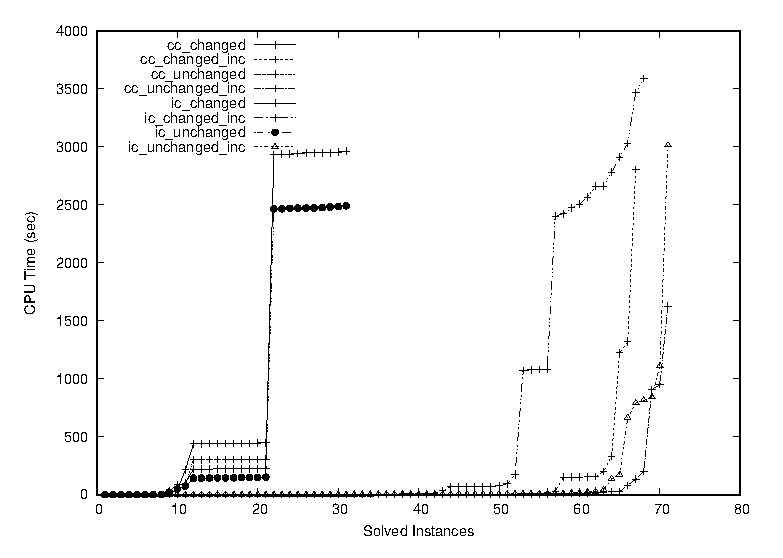
\includegraphics[scale=0.5]{fig/cactus.eps}
  \caption{トポロジ制約のASP符号化の比較 (カクタスプロット)} 
  \label{fig:cactus}
\end{figure*}
%%%%%%%%%%%%%%%%%%%%%%%%%%%%%%
\begin{table*}[t]
  \caption{トポロジ制約のASP符号化の比較 (解けた問題数)} 
  \label{table:kibo}
  \centering
  \begin{tabular}[t]{rcr|c|ccc}
    \noalign{\hrule height 1pt}
    \multicolumn{3}{c|}{スイッチ数} & 問題数 & 基本符号化 & 改良符号化 & 有向符号化\\
    \noalign{\hrule height 1pt}
    %%%%%%%% 
       1 &~& 1000 & 30 & \textbf{30} & \textbf{30} & \textbf{30} \\ 
    1001 &~& 4000 & 20 & \textbf{20} & \textbf{20} & \textbf{20} \\ 
    4001 &~& 7000 & 11 & 9 & \textbf{10} & \textbf{10} \\ 
    7001 &~& 10000 & 8 & 4 & 6 & \textbf{8}  \\ 
    10001 &~& 20000 & 9 & 2 & 5 & \textbf{9} \\ 
    20001 &~& 30000 & 2 & 1 & \textbf{2} & \textbf{2} \\ 
    30001 &~& 40000 & 1 & 0 & 0 & \textbf{1} \\
    40001 &~& 50000 & 4 & 0 & 2 & \textbf{4} \\
    %%%%%%%% 合計
    \noalign{\hrule height 1pt}
    \multicolumn{3}{c|}{計} & 85 & 66 & 75 & \textbf{84} \\
    \noalign{\hrule height 1pt}
  \end{tabular}
\end{table*}
%%%%%%%%%%%%%%%%%%%%%%%%%%%%%%
\begin{table}[tb]
 \centering
 \caption{全解列挙の結果}
 \label{table:enum}
\begin{tabular}[t]{c|c|r|r}
 \noalign{\hrule height 1pt}
 問題名 & $J_i^{max}$ & \multicolumn{1}{|c}{総CPU時間} & \multicolumn{1}{|c}{総数} \\
 \noalign{\hrule height 1pt}
 %%%%%%%%
 %test & 200 & 0.008 & UNSAT \\
 test & 250 & 0.026 & 45 \\
 & 300 & 0.060 & 114 \\
 & 400 & 0.009 & 279* \\ \hline
 %baran32 & 300 & 0.013 & UNSAT \\
 baran32 & 350 & 0.116 & 50751* \\ \hline
 fukui-tepco & 300 & TO~(5日) & 358億+  \\
 \noalign{\hrule height 1pt}
\end{tabular}
\end{table}
%%%%%%%%%%%%%%%%%%%%%%%%%%%%%%



%%% Local Variables:
%%% mode: japanese-latex
%%% TeX-master: "paper"
%%% End:
